\section{Regret Analysis}

Recall from \ref{ch:LiteratureReview} that the cumulative regret of the UCB1 algorithm is proportional to log($n$), where $n$ is the number of plays. Thus, we should expect the UCB1-AKSB algorithm to result in a cumulative pseudo-regret that is approximately logarithmic in the number of plays. This empirical pseudo-regret, $\hat{R}_n$, was calculated using \ref{eq:RegretComputation} below under the assumptions that the long-term average de-anonymization proportion was optimal.

\begin{equation}
\label{eq:RegretComputation}
\hat{R}_n = \mu^{*}n - \sum_{t=1}^{n}{X_{I_t, t}}
\end{equation}

In \ref{eq:RegretComputation}, $\mu^{*}n$ is the expected optimal number of de-anonymizations by play $n$ (i.e. $\max_{i=1,...,K}{\mathbb{E}\left[\sum_{t=1}^{n}{X_{i, t}}\right]}$ from \ref{eq:PseudoRegret}). The plot of $\hat{R}_n$ as a function of $n$ for the UCB1-AKSB algorithm is shown below in \ref{fig:TADe-AnonymizationRegret}.

\begin{figure}[htb]
\centering
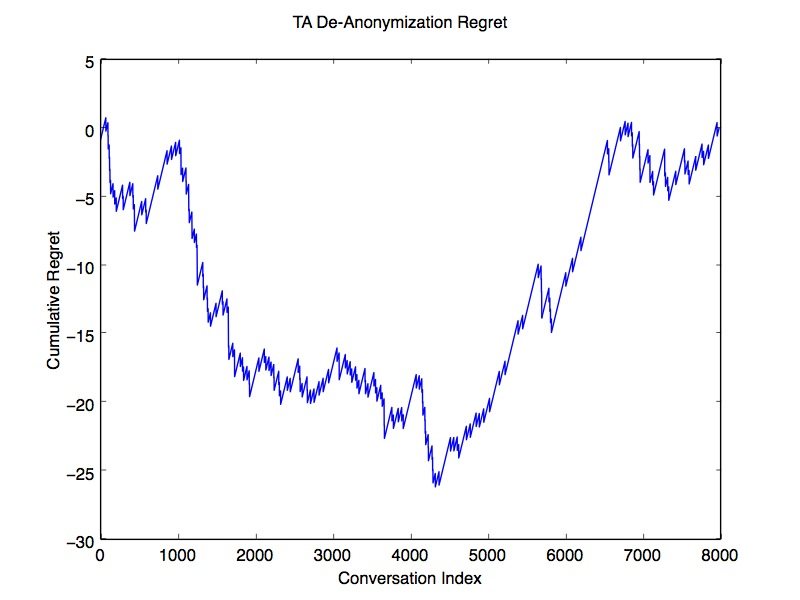
\includegraphics[trim= 0mm 0mm 0mm 0mm, clip, scale=0.5]{./Figures/TADe-AnonymizationRegret.jpg}
\caption{TA De-Anonymization Regret Analysis}
\label{fig:TADe-AnonymizationRegret}
\end{figure}

The regret looks approximately logarithmic for the second half of the dataset, but the first half of the data gives a steadily negative cumulative regret. This is due to the fact that the I.I.D assumption of conversation de-anonymization is most-likely false. Instead, there were probably different regimes in which people perceived Facebook de-anonymization differently. This is most analogous to the Markovian bandits in \cite{bubeck12}, where each conversation starter (i.e. bandit arm) is associated with a Markov process with a discrete set of distributions.

Because of the clear split in the data, it seems like there were two discrete distributions from which de-anonymizations were drawn. The first distribution occurred in the initial stages of TA's launch, where users were more likely to de-anonymize a conversation simply because of the novelty of doing so. This is supported by looking at the initial cumulative Facebook de-anonymization statistics (see \ref{fig:TADe-AnonymizationCumulative}), where the Facebook connect rate was almost double the long-term average. The second distribution most likely occurred as users became more used to the idea of Facebook de-anonymization, the rate of de-anonymization drifted slowly back towards the long term average (around the second half of the data set). The existence of multiple regimes explains the two polar opposite segments of regret data.

\begin{figure}[htb]
\centering
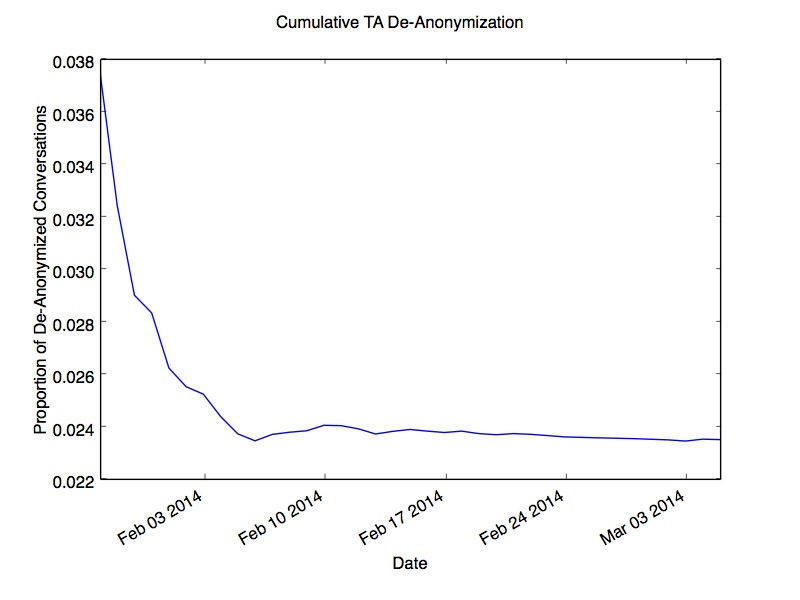
\includegraphics[trim= 0mm 0mm 0mm 0mm, clip, scale=0.5]{./Figures/CumulativeTADe-Anonymization.jpg}
\caption{TA Cumulative De-Anonymization Data}
\label{fig:TADe-AnonymizationCumulative}
\end{figure}

\section{UCB1-AKSB Effectiveness}

Since conversation de-anonymization was the metric used to measure the desirability of each bandit arm, the obvious way to judge the performance of the UCB1-AKSB algorithm is the proportion of conversations which were de-anonymized. Judging from not only the cumulative de-anonymization proportion (\ref{fig:TADe-AnonymizationCumulative}), but also the daily de-anonymization proportion (\ref{fig:TADe-AnonymizationDaily}), it seems that the algorithm had little impact on whether or not people opted to de-anonymize the conversation. 

However, this may have been due to the fact that the user's decision to de-anonymize the conversation was based on factors other than the conversation starter. It is easy to imagine a case in which the conversation was extremely revealing and thus users were hesitant to reveal their identities for fear of being connected to the conversation. In such cases, the conversation starter may have been excellent (and would have led to de-anonymization in most conversation cases), but in certain cases, the tendencies of the specific users would take the conversation in a different direction. In other words, the process of conversation de-anonymization might have been more user-specific (i.e. context dependent) than the UCB1-AKSB algorithm assumed. 

Moreover, even if the process of conversation de-anonymization was sufficiently user-independent for the UCB1-AKSB algorithm to work properly, the metric itself is not granular to accurately measure incremental improvements. For example, let's say the conversation de-anonymization would only occur if the conversation "quality" metric was above some threshold $d$. Even if the UCB1-AKSB algorithm boosted the quality of otherwise low-quality conversation by providing some common ground, such a quality boost would not be visible unless the incremental improvement was enough to make such conversations pass the threshold $d$. Basically, it is entirely possible that the UCB1-AKSB algorithm could improve conversation quality but this increased likelihood would not be visible because of the censoring nature of the threshold hypothesized above. This threshold hypothesis would also explain the erratic de-anonymization rate seen in \ref{fig:TADe-AnonymizationDaily}.

\begin{figure}[htb]
\centering
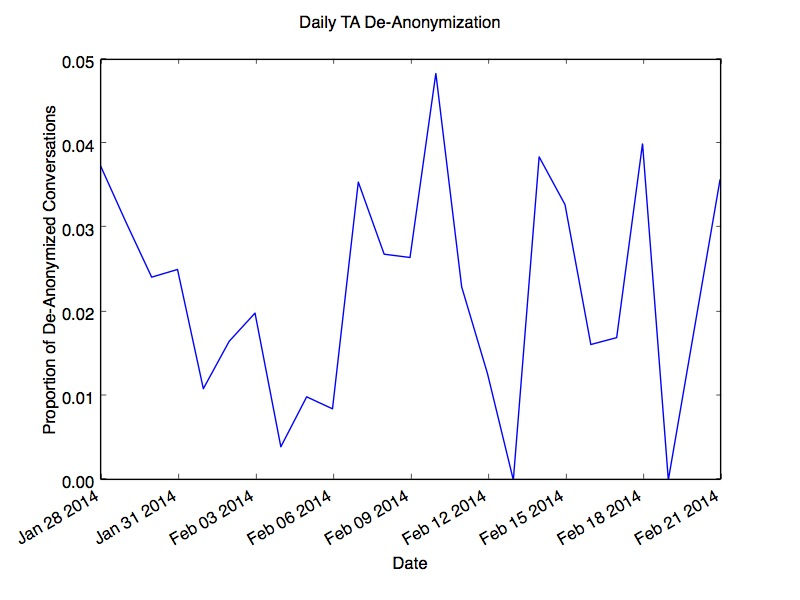
\includegraphics[trim= 0mm 0mm 0mm 0mm, clip, scale=0.5]{./Figures/DailyTADe-Anonymization.jpg}
\caption{TA Daily De-Anonymization Data}
\label{fig:TADe-AnonymizationDaily}
\end{figure}

Given that conversation de-anonymization might have been affected by other exogenous variables and was not granular enough to measure incremental improvements in conversation quality, it makes sense to turn to other conversation quality metrics to judge the performance of the algorithm. These other metrics (participation rates and average conversation rates) are less likely to be influenced by the social pressure for or against de-anonymization, as well as having a more finely differentiated set of values than the binary variable of conversation de-anonymization. The plots of both these metrics are shown below in \ref{fig:TAParticipationCumulative} and \ref{fig:TAMessagesExchangedCumulative}.

\begin{figure}[H]
\centering
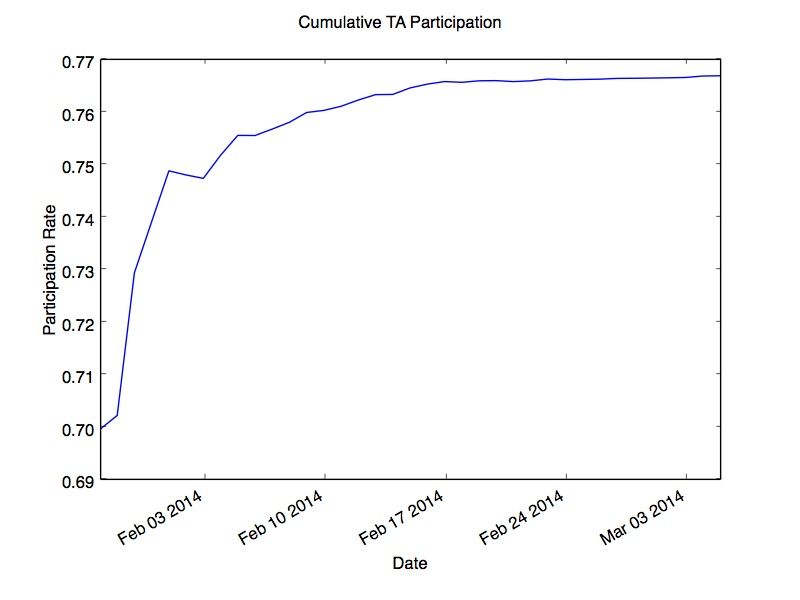
\includegraphics[trim= 0mm 0mm 0mm 0mm, clip, scale=0.5]{./Figures/CumulativeTAParticipation.jpg}
\caption{TA Cumulative Participation Rate}
\label{fig:TAParticipationCumulative}
\end{figure}

\begin{figure}[H]
\centering
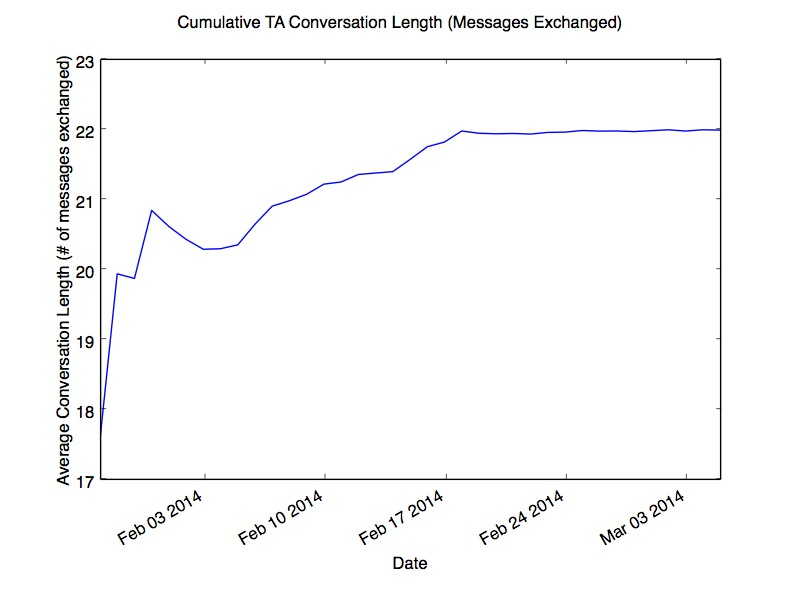
\includegraphics[trim= 0mm 0mm 0mm 0mm, clip, scale=0.5]{./Figures/CumulativeTAConversationLength(MessagesExchanged).jpg}
\caption{TA Cumulative Average Conversation Length}
\label{fig:TAMessagesExchangedCumulative}
\end{figure}

By these metrics, it seems that conversation quality improved noticeably over the course of the user experience, which suggests that the UCB1-AKSB algorithm may have had a positive effect on conversation quality even though some of its fundamental assumptions weren't true.

\section{Individual User Analysis}

Another way of examining the data is to look at how individual users as they continued to interact with the site. In each of the plots below, the x-axis represents the number of uses, while the y-axis represents the conditional mean of the metric over the set of users on the $n$-th use, given that they've used the site greater than or equal to n times. In order to define this more formally, I introduce the following notation: let $f_k(u, n)$ give the value of conversational quality metric $k$ for user $u$ on their $n$-th visit and function $g(u)$ give the number of times user $u$ has visited the site. Let $U_n$ be the set $\{u | u \in {U}, g(u) \geq{n}\}$ (i.e. the set of users who have visited the site at least $n$ times). Then, the graphs below are plots of the following functions $y_k(n)$ for different conversational quality metrics $k$.

$$ y_k(n) = \frac{1}{|U_n|}\sum_{u \in U_n}{f_k(u, n)} $$

\begin{figure}[H]
\centering
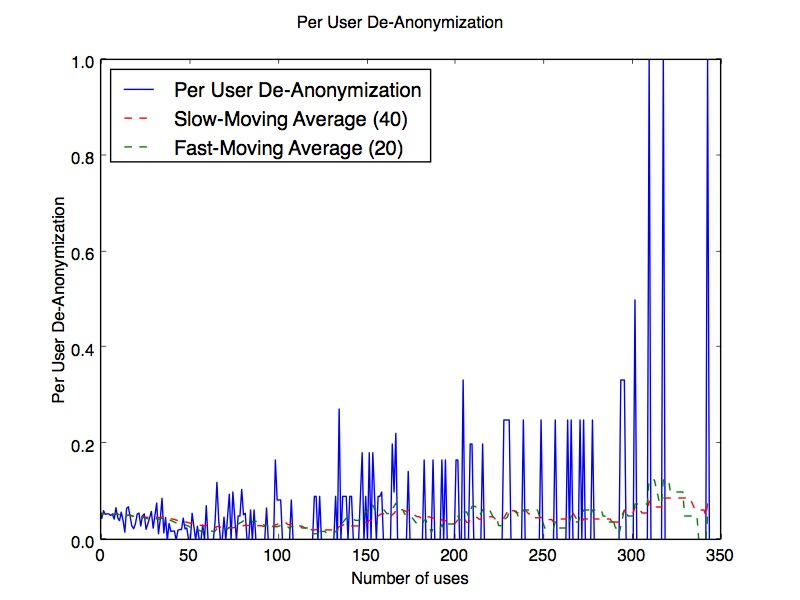
\includegraphics[trim= 0mm 0mm 0mm 0mm, clip, scale=0.5]{./Figures/PerUserDe-Anonymization.jpg}
\caption{Per User De-Anonymization Proportion}
\label{fig:PerUserFBConnect}
\end{figure}

\begin{figure}[H]
\centering
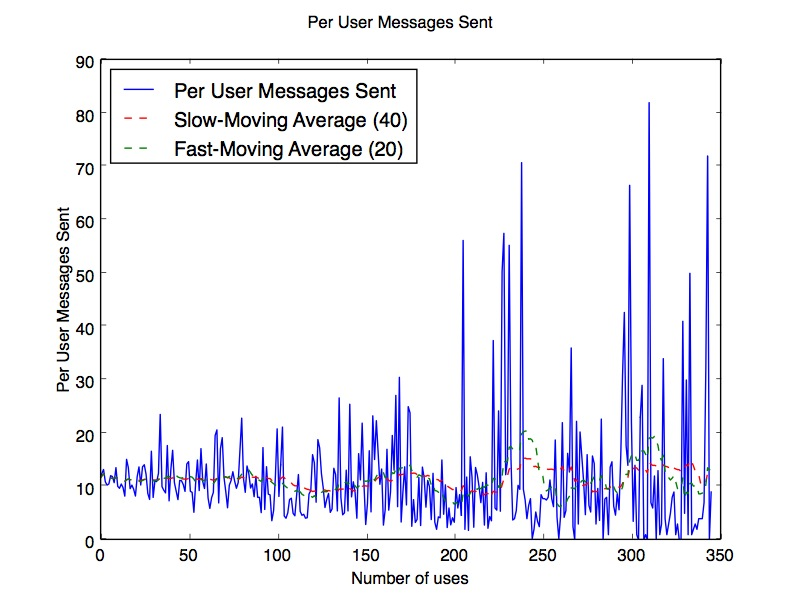
\includegraphics[trim= 0mm 0mm 0mm 0mm, clip, scale=0.5]{./Figures/PerUserMessagesSent.jpg}
\caption{Per User Messages Sent}
\label{fig:PerUserMessagesSent}
\end{figure}

\begin{figure}[H]
\centering
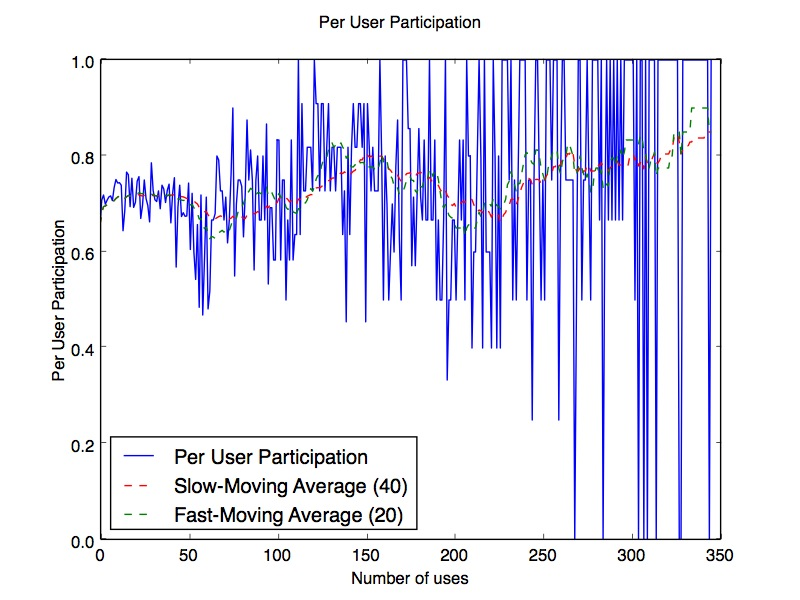
\includegraphics[trim= 0mm 0mm 0mm 0mm, clip, scale=0.5]{./Figures/PerUserParticipation.jpg}
\caption{Per User Participation}
\label{fig:PerUserParticipation}
\end{figure}

The two things that immediately stand out about these plots are the general upward drift over time and increasing volatility over time. The general upward drift of each conversation quality metric on a user-level can be explained by a combination of two factors: the UCB1-AKSB algorithm is selecting better conversation starters for each user as they use the site more frequently, and the users who return to the site frequently are more likely to have higher quality conversations simply because of their status as "power users". Second, the increasing volatility over time of each conversation quality metric represents the stratification of users into different classes. An abrupt change from a participation rate of 100 percent to 0 in one turn is more likely the result of a "power user" being paired with an first-time user, so that the first-time user disconnects from the conversation before the "power user" has a chance to participate at all.

This high volatility (and the user stratification it represents) raises the issue of user saturation: people were either hooked and used the site extremely frequently or they used it a few times and then left. WE WANT A MIDDLE CLASS, A SET OF CASUAL USERS WHO ARE INVOLVED ENOUGH TO TAKE IT SERIOUSLY BUT CASUAL ENOUGH SO THAT IT'S REALISTIC TO HAVE A LARGE NUMBER OF THEM. Since Princeton is such a small sample pool, this is why I'm currently working on a larger version of Tigers Anonymous (with a working title of Campus Anonymous) that will be released to a small subset of schools, thus allowing the site to have access to a much broader user base, and thus a much higher likelihood of attracting a non-trivial set of casual users.
